\documentclass[letterpaper,10pt,twocolumn,titlepage]{article}

\usepackage{graphicx}
\usepackage{amssymb}
\usepackage{amsmath}
\usepackage{amsthm}

\usepackage{alltt}
\usepackage{url}

\usepackage{multicol}

\usepackage{geometry}
\geometry{textheight=8.5in, textwidth=6in}

%random comment

\usepackage{hyperref}
\usepackage{geometry}

\def\name{Byron Kropf}

%% The following metadata will show up in the PDF properties
\hypersetup{
  colorlinks = true,
  urlcolor = black,
  pdfauthor = {\name},
  pdfkeywords = {cs311 ``operating systems'' files filesystem I/O},
  pdftitle = {CS 311 Project 1: File I/O},
  pdfsubject = {CS 311 Project 1},
  pdfpagemode = UseNone
}
\title{CS 311 Project 1: File I/O}
\date{January 20, 2012}
\author{Byron Kropf}
\maketitle
\sloppy
\begin{document}
\section{Introduction}
In this assignment we were tasked to create a program in C to copy an arbitrary file from one place to another, in order to learn about the use of a few basic system calls in Linux. Our program should create the file to copy to and not overwrite any existing file. We used the open(), close(), read(), and write() system calls in order to implement the program, and the time utility to time runtimes using varying buffer sizes to chart the relationship to buffer size and the time it takes to copy a file.

\section{Assignment 1: Copy a File}
\subsection{open() and close()}
The open() and close() system calls are used to open and close file descriptors. The open() function opens a file so that it may be read from or written to, and returns the integer value of a newly opened file descriptor or -1 if there is an error. The function takes two arguments. The first argument is a pointer to a character array of the pathname of the file to be opened. The second argument is a set of flags that control access permissions for the opened file.Calling close() is necessary when we are done with an open file in order to free up its descriptor. It returns 0 on success, and -1 on failure.

\newLine
\newLine

The first time we call open we only use the O\_RDONLY flag while opening the file we will copy from. As expected this flag opens the file in read-only mode and prevents us from altering our source file as it is being copied to the destination.The second time we call open() we add a few different flags so that we can work with the destination file. Namely these flags are O\_APPEND, O\_CREAT, O\_EXCL, and O\_WRONLY. The O\_APPEND and O\_WRONLY flags are obvious in order to avoid copying over any existing data. The O\_CREAT lets open() create a new file if the requested file does not exist, and the O\_EXCL flag stops us from using an alread exsisting file.

\newline
\newline

\subsection{read() and write()}
As opposed to the first two calls we used which simply open and close files, read() and write() perform the bulk of the copy operation. The system call read() takes an open file descriptor, a buffer to read into, and the number of characters to read. On success it returns the number of read characters. When there is an errr it returns -1, and when the end of the file is reached it returns 0. The write function recieves the same arguments for slightly different purposes, most notably it reads from the buffer and writes to the file, rather than reading the file and writing to the buffer.

\newline
\newline

\section{File System Performance}
\subsection{Testing Methods and Results}
Using bash's time utility I timed the runtime of my program, when copying the file provided by the instructor, using powers of 2 from 1 to 8192 bytes as the buffer size. I used the real time which is the su of both the user and kernal space time. When using a small buffer size the program took longer due to a vastly increased number of system calls being required to finish. Performance was maximized at a buffer size of 4096 which is the block size of my file system. Performance increases using a buffer size larger than 4096 were neglegible for this program.

\newline
\newline

\section{Bibiography}
Kerrisk, Michael. "Chapter 4." The Linux Programming Interface: A Linux and UNIX System Programming Handbook. San Francisco: No Starch, 2010. Print.

\begin{figure}[h]
  \caption{Results of the timing test}
  \centering
    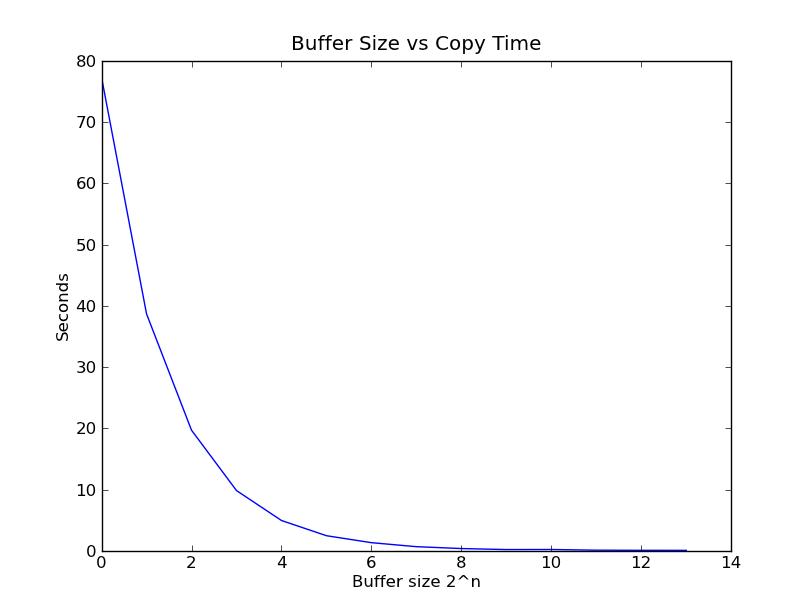
\includegraphics[width=.75\textwidth]{copy_times.png}
\end{figure}
\end{document}
